%\documentclass[border=3mm]{standalone}
%\usepackage{pgfplots}
%\pgfplotsset{compat=newest}
%\pagestyle{empty}
%\begin{document}
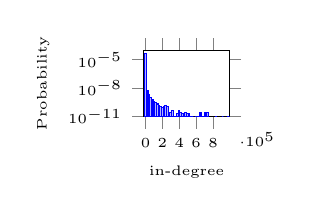
\begin{tikzpicture}
\begin{axis}[ymax=0.0001,ybar,ymode=log,bar width=19880.36,log origin=infty,xmin=-19880.36,ytick align=outside,enlargelimits=0,
width=.22\textwidth,
height=.20\textwidth,
ylabel=Probability,
xlabel=in-degree,
every x tick scale label/.style={at={(xticklabel cs:1)},anchor=south west},
  label style={font=\tiny},
tick label style={font=\tiny} ,
] 
\addplot  plot coordinates {
(0.0, 5.02894342734e-05)
(19880.36, 5.8571821351e-09)
(39760.72, 1.86029998631e-09)
(59641.08, 1.08670989299e-09)
(79521.44, 5.80192569987e-10)
(99401.8, 4.05213858403e-10)
(119282.16, 3.22329205548e-10)
(139162.52, 2.02606929202e-10)
(159042.88, 1.47350493965e-10)
(178923.24, 1.19722276346e-10)
(198803.6, 8.28846528552e-11)
(218683.96, 1.01303464601e-10)
(238564.32, 1.28931682219e-10)
(258444.68, 1.10512870474e-10)
(278325.04, 9.2094058728e-12)
(298205.4, 2.76282176184e-11)
(318085.76, 4.6047029364e-11)
(337966.12, 9.2094058728e-12)
(357846.48, 9.2094058728e-12)
(377726.84, 1.84188117456e-11)
(397607.2, 3.68376234912e-11)
(417487.56, 2.76282176184e-11)
(437367.92, 1.84188117456e-11)
(457248.28, 9.2094058728e-12)
(477128.64, 2.76282176184e-11)
(497009.0, 1.84188117456e-11)
(516889.36, 1.84188117456e-11)
(536769.72, 9.2094058728e-12)
(556650.08, 9.2094058728e-12)
(576530.44, 0.0)
(596410.8, 9.2094058728e-12)
(616291.16, 9.2094058728e-12)
(636171.52, 9.2094058728e-12)
(656051.88, 2.76282176184e-11)
(675932.24, 9.2094058728e-12)
(695812.6, 9.2094058728e-12)
(715692.96, 2.76282176184e-11)
(735573.32, 2.76282176184e-11)
(755453.68, 0.0)
(775334.04, 0.0)
(795214.4, 0.0)
(815094.76, 0.0)
(834975.12, 9.2094058728e-12)
(854855.48, 0.0)
(874735.84, 0.0)
(894616.2, 0.0)
(914496.56, 9.2094058728e-12)
(934376.92, 0.0)
(954257.28, 0.0)
(974137.64, 9.2094058728e-12)
(994018.0, 9.2094058728e-12)
};\end{axis}
\end{tikzpicture}
%\end{document}